\documentclass[NUS-Kajima workshop]{beamer}
\usetheme{Boadilla}
\usepackage{essay-def}
\usepackage{bm}
\usepackage{amsfonts}
\usepackage{amssymb}
\usepackage{amsmath}
\usepackage{amsthm}
\usepackage{comment}
\usepackage{subcaption}
\usepackage{geometry}
\usepackage{algorithmic}
\usepackage{algpseudocode}
\usepackage{algorithmicx}
\geometry{left=1cm,right=1cm}
    \title[Mitigating DS in SciML]{Mitigating distribution shift in machine learning-augmented hybrid simulation\footnotemark}
\author[J. Zhao]{Jiaxi Zhao (NUS) \\ \small joint work with Prof. Qianxiao Li (NUS)}
\date[\today]{The 13th Symposium of the SIAM Student Chapter@NUS \\ \today}
\begin{document}
\par \setlength{\parindent}{2em}

\begin{frame}
\titlepage
\footnotetext[1]{https://arxiv.org/abs/2401.09259}
\end{frame}


\begin{frame}{Practical scientific problems}
	\begin{figure}[ht]
		\centering
		\begin{subfigure}{0.5\linewidth} % Adjust the width as needed
			\centering
			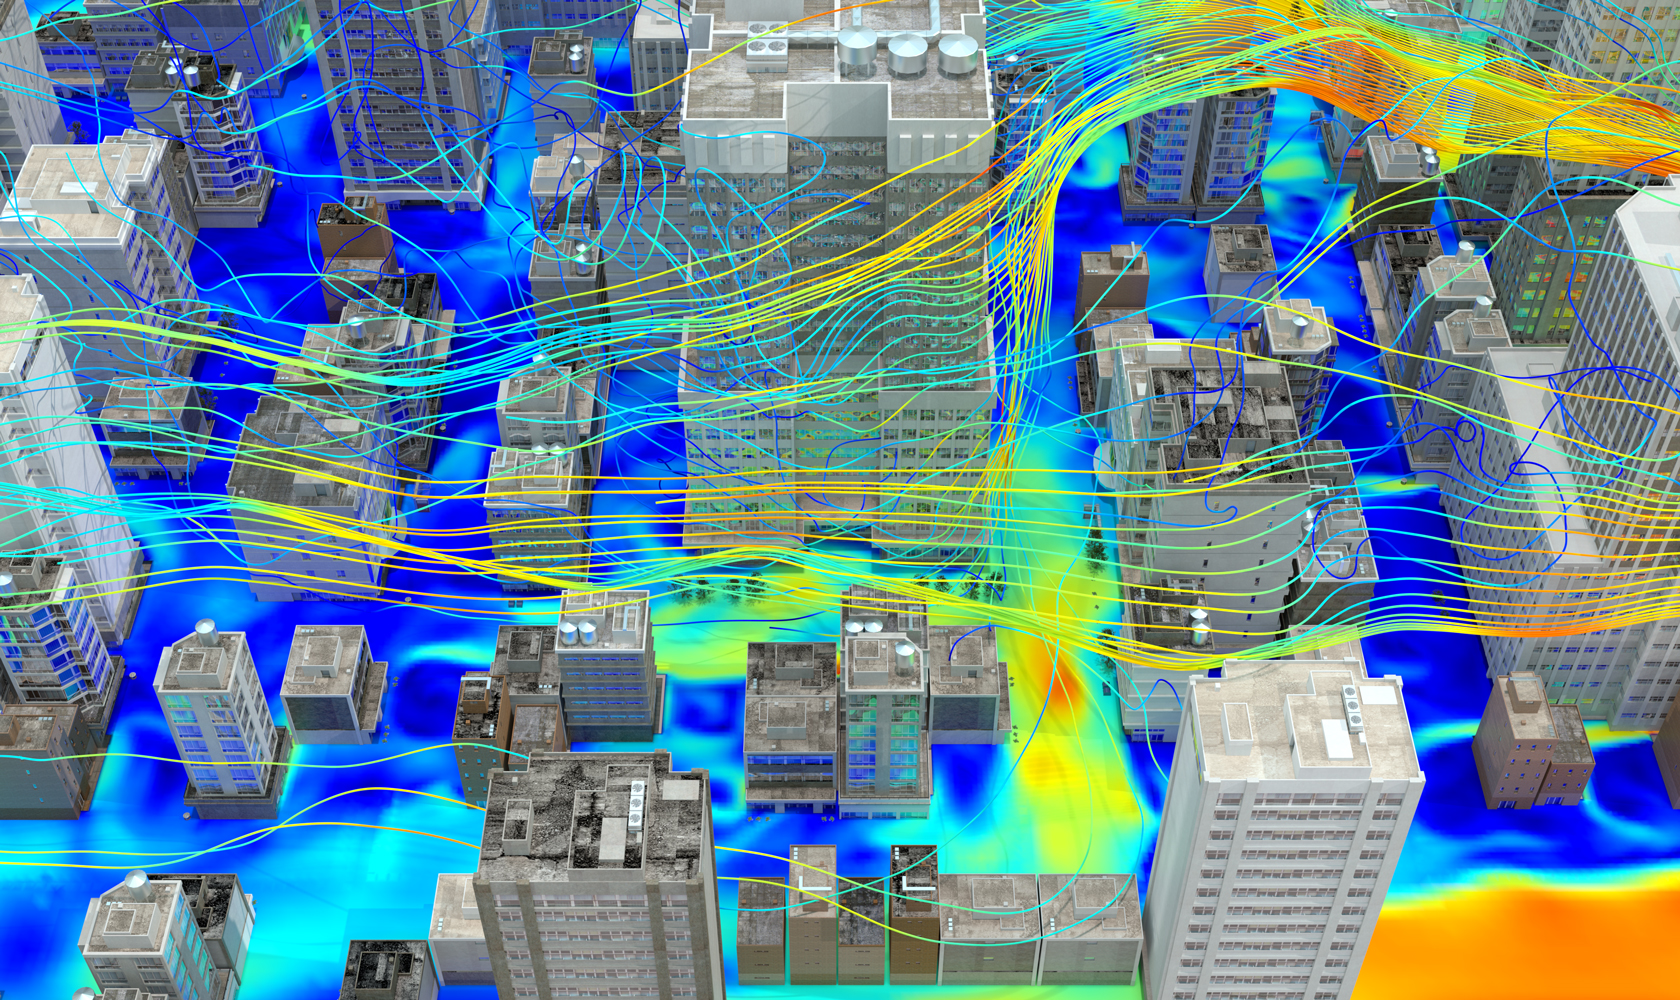
\includegraphics[width=\linewidth]{fig/urban_environment.jpeg}
			\caption{Computational fluid dynamics for urban environment}
		  \end{subfigure}%
		  \begin{subfigure}{0.5\linewidth} % Adjust the width as needed
			\centering
			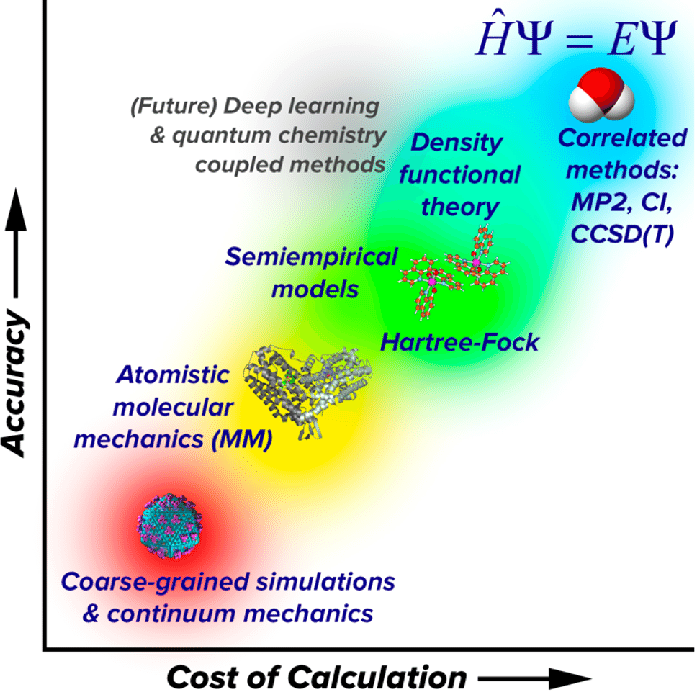
\includegraphics[width=\linewidth]{fig/quantum_chemisty.png}
			\caption{Quantum chemistry for material science}
		  \end{subfigure}
	\end{figure}
\end{frame}


\begin{frame}{Data-driven scientific computing}
	\textbf{What are the problems we are interested in?}
	\begin{itemize}
		\item 1. {\color{red}Forward problem: Increase the stability and accuracy of machine learning-augmented simulation.}
		\item 2. Inverse problem: Learn the surrogate models and Perform effective sensitivity analysis to do inverse designs. 
	\end{itemize}

	\textbf{What are methods we focus on?}
	\begin{itemize}
		\item 1. 100\% data-driven: AlphaFold series, FermiNet, Fourier neural operator, DeepONet.
		\item 2. {\color{red}50 \% Numerical + 50 \% data-driven: Machine learning turbulence modeling, force fields, exchange-correlation functionals.}
	\end{itemize}
\end{frame}

\begin{frame}{A Framework for the hybrid approach}
	Simulating the dynamics:
	\bequn
		\begin{aligned}
			\p_t \mfx & = \mcL(\mfx, \mfu, t), \quad \mfx \in \mcX, \mfu \in \mcU, \mcL: \mcX \times \mcU \times \mbR_+ \rightarrow T\mcX,			\\
			\mfu & = \phi(\mfx, t), \quad \phi: \mcX \times \mbR_+ \rightarrow \mfu.
		\end{aligned}
	\eequn
	\begin{itemize}
		\item 1. $\mcL$ is known, possibly non-linear.
		\item 2. $\phi$ is un-known.
		\item 3. A set of data pairs $\lbb (\mfx_1, \mfu_1, t_1), (\mfx_2, \mfu_2, t_2), \cdots, (\mfx_N, \mfu_N, t_N )\rbb. $
		\item 4. {\color{red}Benchmark algorithm solves the ordinary least square:
		\bequn
			\arg\min_{\theta} \mbE \norml \mfu - \phi_{\theta}(\mfx, t) \normr^2.
		\eequn}
	\end{itemize}
		{\color{red}Why surrogate models? The dynamics are unknown, nonlinear, computationally expensive etc.}
\end{frame}

\begin{frame}{An example}
	Let us use the incompressible NS equation as an example
	\begin{equation*}
    \begin{aligned}
        	\frac{\p \mfu}{\p t} + (\mfu \cdot \nabla)\mfu -  \nu \Delta \mfu & =   \nabla p, \quad T \in [0, 1], 	\\
		\nabla \cdot \mfu & = 0.
    \end{aligned}
\end{equation*}
Consider solving it using the projection method, in each step, we need to solve the following equation
\bequn
\begin{aligned}
	\mfu_{k+1} 	& = \mfu_k +
	\Delta t (\nu \Delta \mfu_k
	- (\mfu_k \cdot \nabla)\mfu_k - \nabla p_{k}),    \\
	p_{k} & = \phi(\mfu_k) = \Delta^{-1}(\nabla \cdot \lp \nu \Delta \mfu_k
	- (\mfu_k \cdot \nabla)\mfu_k\rp),   \\
\end{aligned}
\eequn

The most important features are: 
\begin{itemize}
	\item 1. {\color{red}iterative solver}
	\item 2. {\color{red}data-driven}
\end{itemize}
\end{frame}

\begin{frame}{Dilemma of data-driven scientific computing}
	In data-driven scientific computing, \textcolor{red}{dynamics itself} can cause \textcolor{red}{distribution mismatch} between the training and testing data.
	Similarly to the \textcolor{red}{extrapolation, out-of-distribution} issue in NLP.
	\begin{figure}[ht]
		\centering
			\centering
			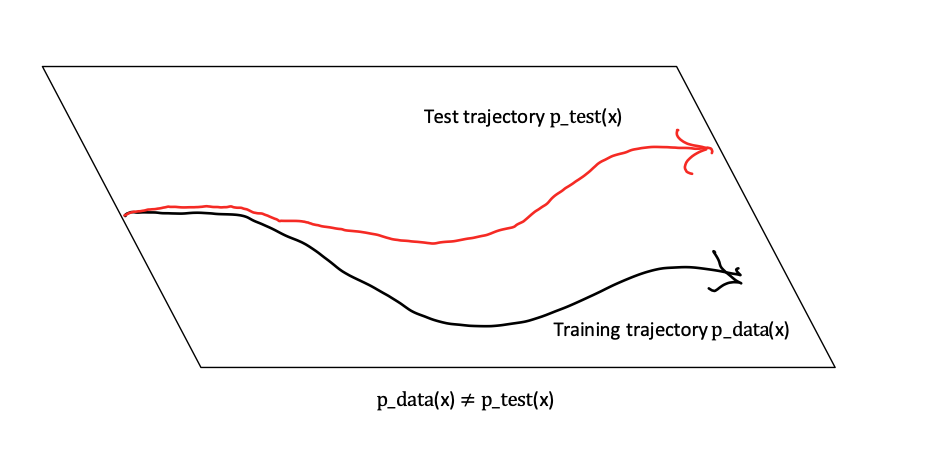
\includegraphics[width=\linewidth]{fig/dilemma.png}
			\caption{Distribution shift illustration}
	\end{figure}
\end{frame}

\begin{frame}{Different from classical numerical stability}
	This is different from the classical numerical stability issue. For the ablation study, we add {\color{red}noises of the same scale to the numerical solver}
	(without the data-driven part) and compare the simulations.
	\begin{figure}[ht]
		\centering
			\centering
			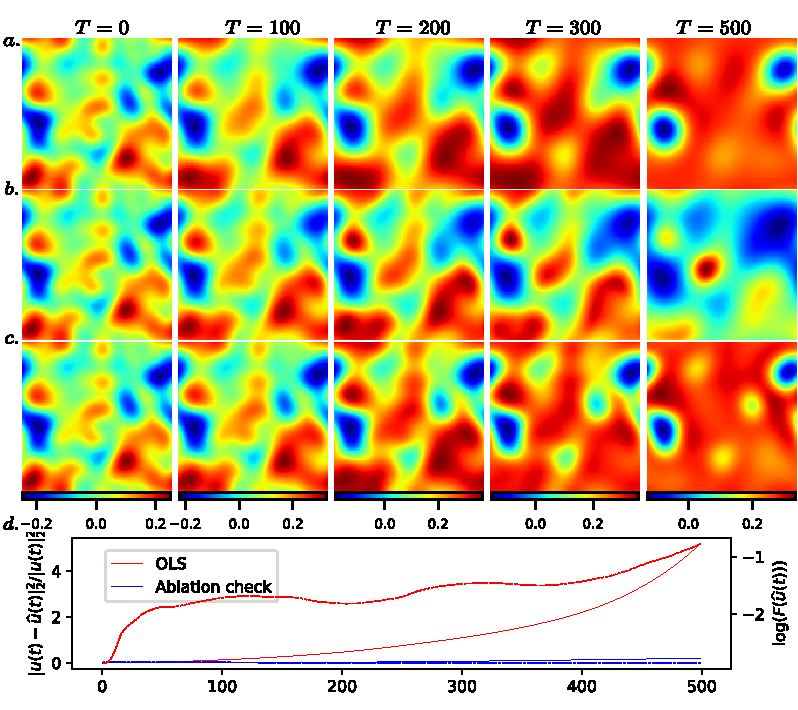
\includegraphics[width=.6\linewidth]{fig/RD-ds.pdf}
			\caption{Distribution shift in reaction-diffusion equation}
	\end{figure}
\end{frame}

\begin{frame}{An heuristic solution}
	\begin{figure}[H]
		\centering
		\centerline{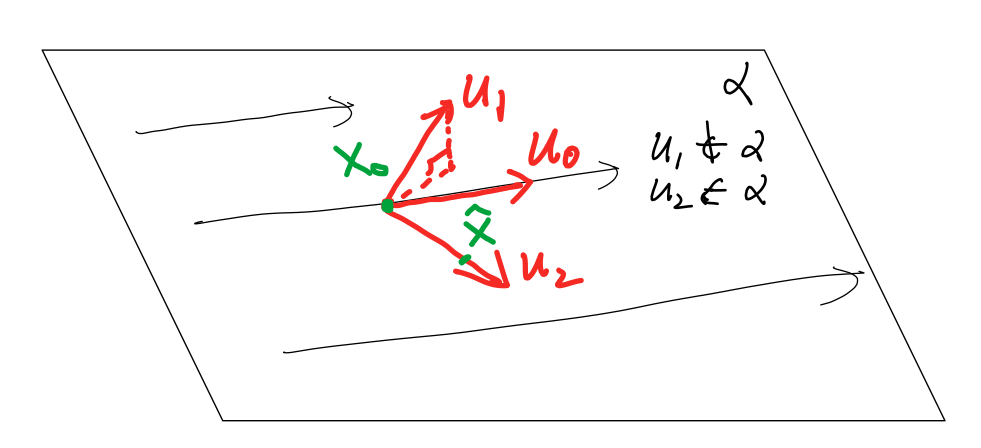
\includegraphics[width=0.9\linewidth]{fig/mfd.png}}
	  \end{figure}
	  We design an algorithm that {\color{red}favors $\mfu_2$ than $\mfu_1$} by adding some regularization.
\end{frame}

\begin{frame}{Linear dynamics}
	We consider the following the \text{\color{red}linear} hybrid simulation problem
	\bequn
		\begin{aligned}
			\frac{d\mfu}{dt} & = A\mfu + B\mfy,  \quad \mfu\in\mbR^m, \mfy \in \mbR^n, A\in \mbR^{m \times m}, B\in \mbR^{m \times n}   \\
			\mfy & = C^* \mfu,  \quad C^* \in \mbR^{n\times m}.
		\end{aligned}
	\eequn
	The least squares estimator aims to minimize the following loss
	\begin{equation*}
		l_{\text{OLS}}(\wht C) = \mbE\norml (\wht C - C^*) \mfu \normr^2,
	\end{equation*}
	while the proposed estimator minimizes
	\begin{equation*}
		l_{\text{TR}}(C) := \mbE_{(\mfu, \mfy)} \lp \norml (\wht C - C^*) \mfu\normr_2^2 + \lambda \norml P_{V^{\perp}}(A + BC)\mfu \normr_2^2 \rp,
	\end{equation*}
\end{frame}

\begin{frame}{Linear theory}
	The tangent-space regularized estimator {\color{red}performs a weighted least squares}
	\begin{Prop}
		Given a data matrix $\mfU \in \mbR^{m \times N}$ with observation noise $\epsilon$ of the same shape 
		\begin{equation*}\label{estimator-formula}
			\begin{aligned}
			\wht C_{\text{OLS}} = & \ C^* P_V + \epsilon \mfU^{\dagger},    \\
			\wht C_{\text{TR}} = & \ (\mfI + \lambda B^T P_{V^{\perp}} B)^{-1}(C^* P_V + \epsilon \mfU^{\dagger} - \lambda B^T P_{V^{\perp}} AP_{V}).
			\end{aligned}
		\end{equation*}
	\end{Prop}
	Specifically, in the noiseless scenarios, we have
	\begin{equation*}
		\wht C_{\text{OLS}} = & \ C^* P_V, \quad \wht C_{\text{TR}} = (\mfI + \lambda P_{V^{\perp}})^{-1}(C^* P_V + \epsilon \mfU^{\dagger})= (\mfI + \lambda P_{V^{\perp}})^{-1}\wht C_{\text{OLS}}.
	\end{equation*}
\end{frame}

\begin{frame}{Linear theory}
	The tangent-space regularized estimator has {\color{red}slower error scaling for large $\lambda$}:
	\begin{Thm}
		With $Q_m(r, T)$ defined by $m^2\int_0^T (2 + t^{m-1})e^{r t}dt$ and
		\begin{equation*}
			\begin{aligned}
				e_1 = \text{eig}_{\max}(A+B\wht C), \quad e_2 = \text{eig}_{\max}((A+B\wht C)P_V), \\
				\text{eig}_{\max}(A) = \max\{\Re(s): \exists v \neq \mathbf{0}, Av = sv\},
			\end{aligned}
		\end{equation*}
		the errors of OLS and our algorithm are bounded respectively by
		\begin{equation*}\label{equ:a-posterior-error}
			\begin{aligned}
				& \ \mbE\norml \wht\mfu_{\text{OLS}}(T) - \mfu(T) \normr \leq c_1\sqrt{\delta}\norml B \normr_2Q_m(e_1, T),      \\
				& \ \mbE\norml \wht\mfu_{\text{TR}}(T) - \mfu(T) \normr \leq c_2\sqrt{\delta}\Big(\norml B \normr_2 Q_m(e_2, T) \\
			& + \frac{9m^4c_3}{\sqrt{\lambda}}\lp 1 + 3m^2c_1\sqrt{\delta}\norml B \normr_2\rp\norml A+B\wht C \normr_2 (1\vee T^{3m})(1\vee e^{e_1T}) \Big).
			\end{aligned}
		\end{equation*}
	\end{Thm}
\end{frame}

\begin{frame}{Linear experiments}
	Consider a linear synthetic dynamics where the data subspace $V(V^{\perp})$ is the stable (unstable) manifold.
	\begin{figure}[ht]\label{fig:linear-cmp}
		\centering
		\centerline{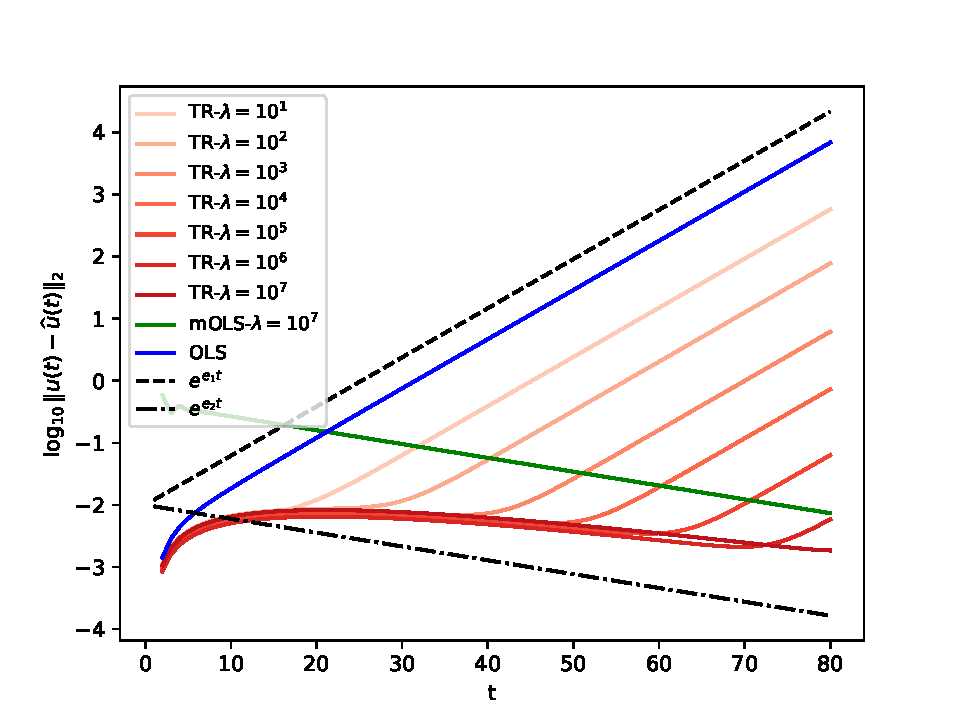
\includegraphics[width=.8\linewidth]{fig/exp2-1.pdf}}
		\caption{Linear synthetic dynamics}
	\end{figure}
\end{frame}

\begin{frame}{Overall algorithm}
	\textbf{Use an autoencoder to parametrize the nonlinear data-manifold.}
	\begin{figure}
		\centering
		\centerline{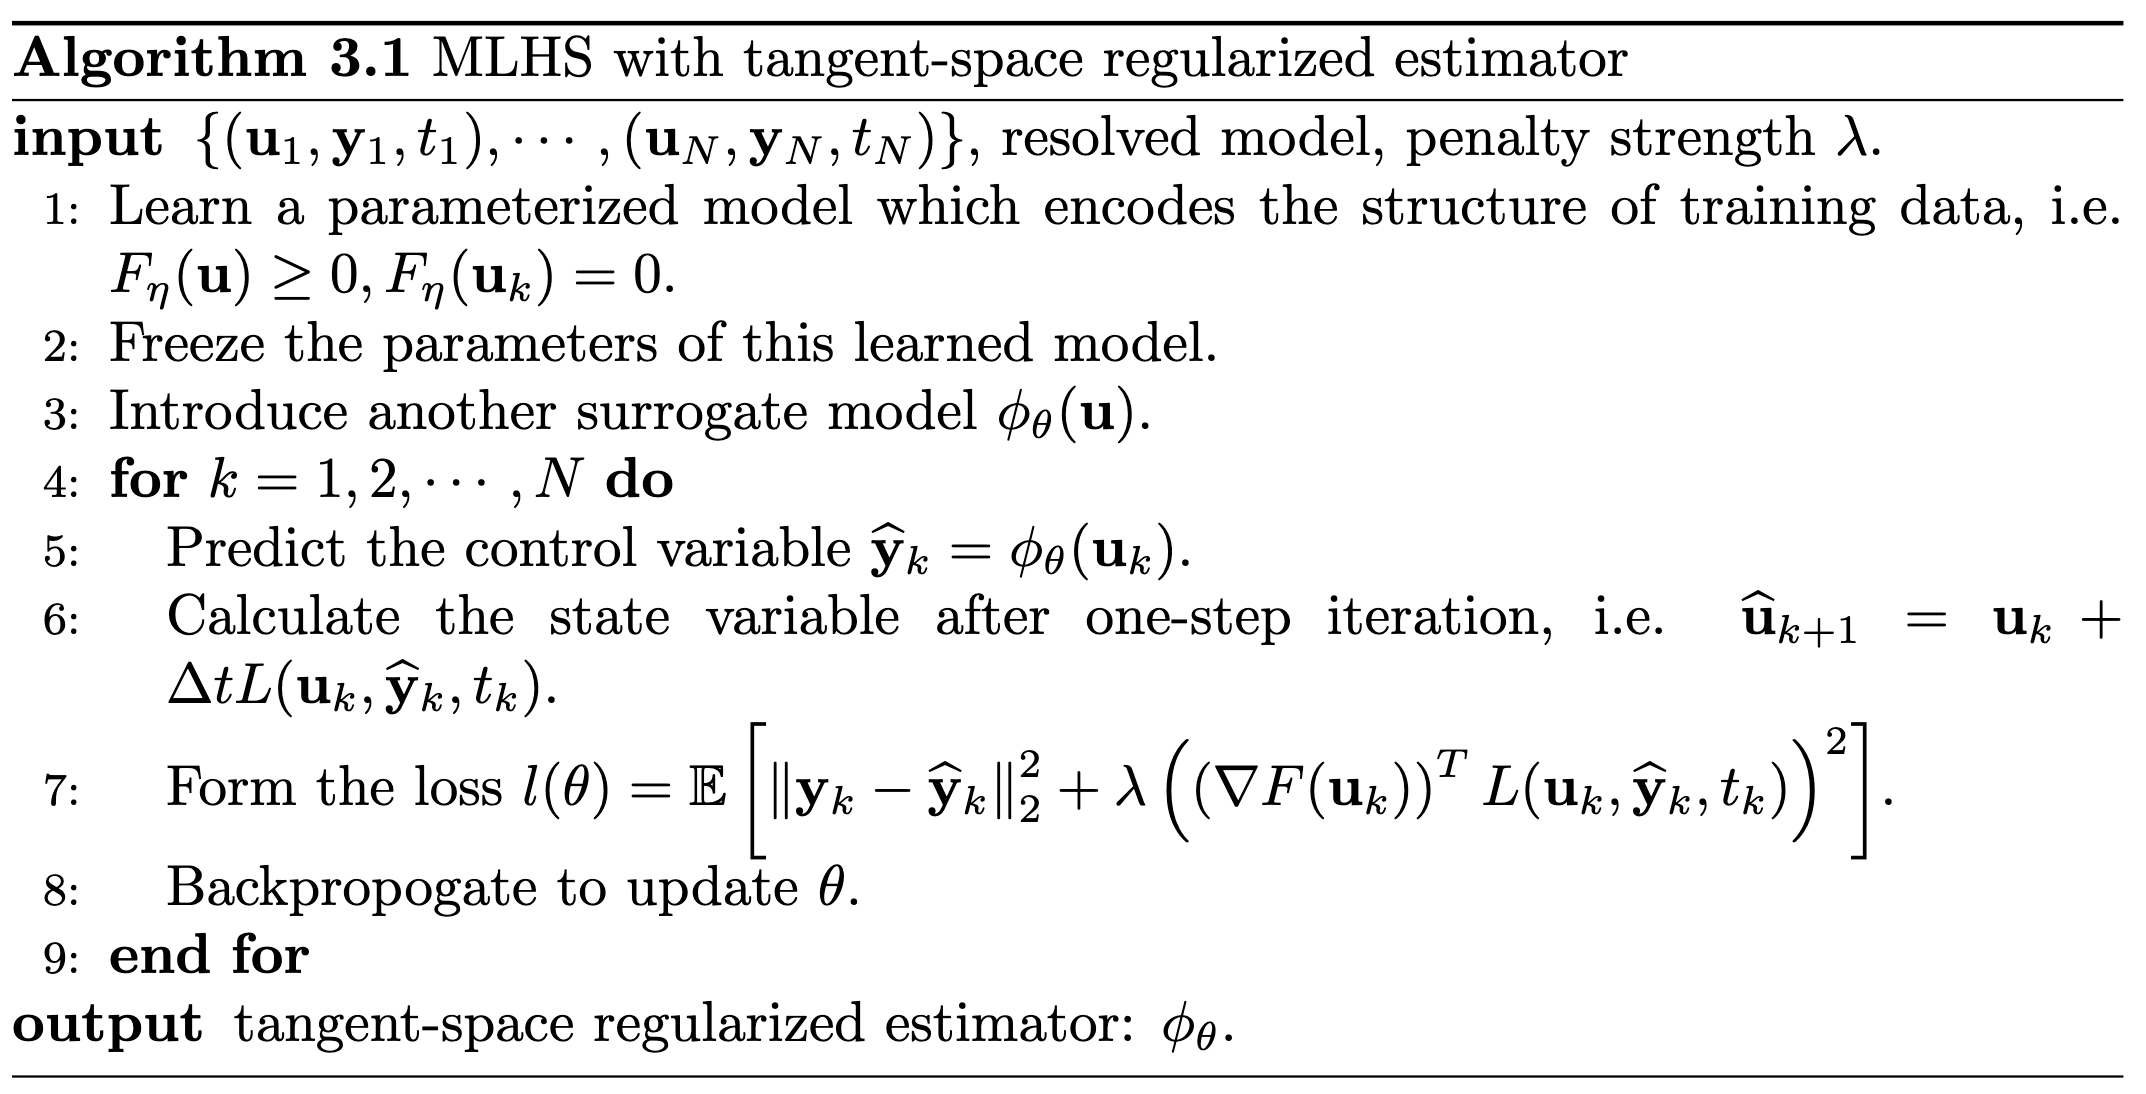
\includegraphics[width=\linewidth]{fig/alg.jpg}}
		\caption{Algorithm pseudocode}
	  \end{figure}
\end{frame}

\begin{frame}{Network architecture}
	We choose U-net for 
	\begin{figure}[H]
          \centering
          \centerline{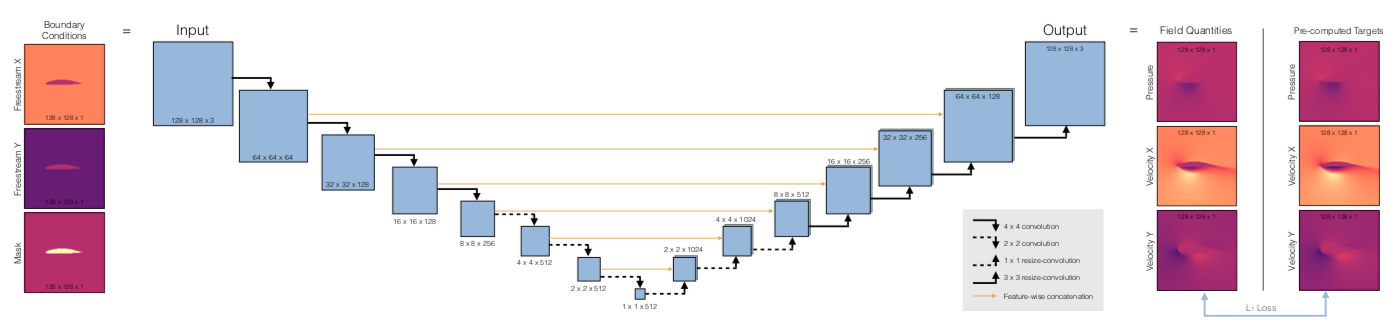
\includegraphics[width=1.1\linewidth]{fig/Unet.png}}
          \caption{U-net structure for flow prediction\footnotemark}
\end{figure}
\footnotetext{Thuerey, Nils, et al. "Deep learning methods for Reynolds-averaged Navier–Stokes simulations of airfoil flows." AIAA Journal 58.1 (2020): 25-36.}
\end{frame}

\begin{frame}{Performance comparison}
	\begin{figure}[H]
          \centering
          \centerline{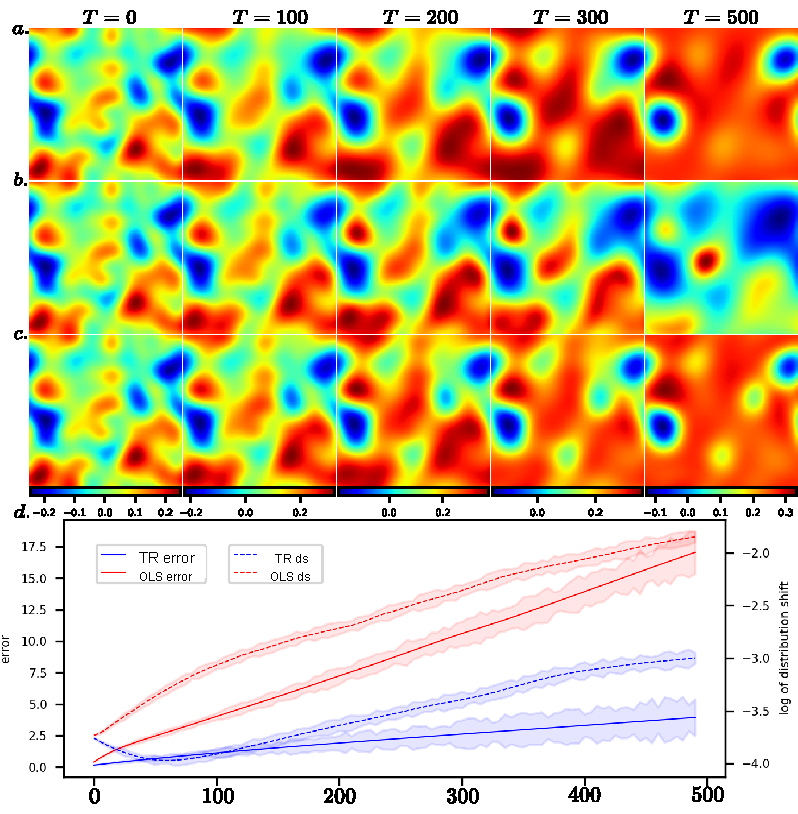
\includegraphics[width=.7\linewidth]{fig/RD-TR.pdf}}
          \caption{Comparison of our method and naive method}
\end{figure}
\end{frame}

\begin{frame}{Performance comparison}
	\begin{figure}[H]
          \centering
          \centerline{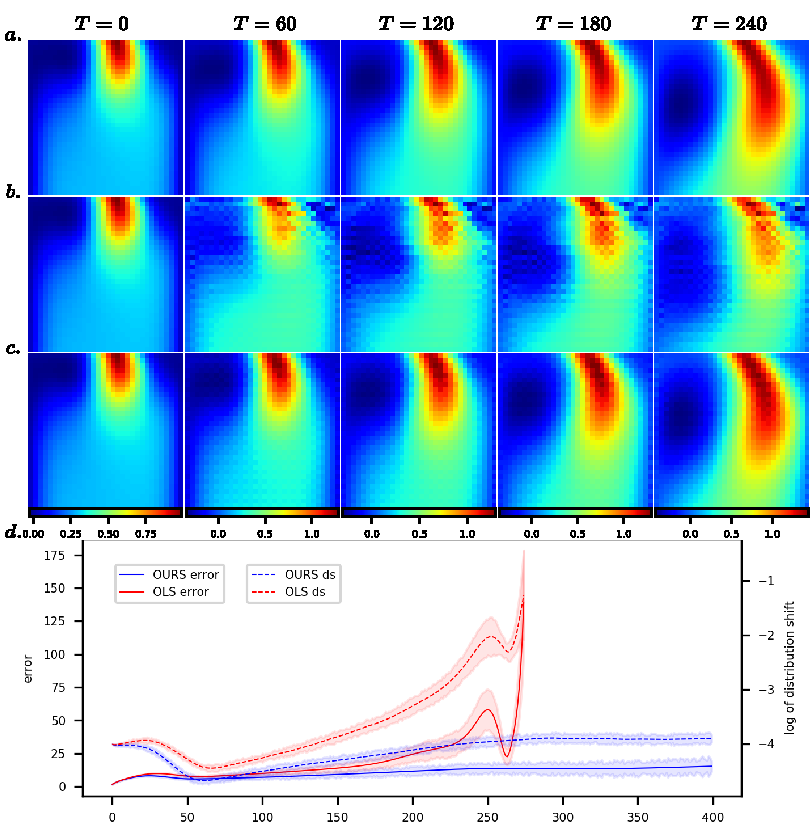
\includegraphics[width=.7\linewidth]{fig/NS-TR.pdf}}
          \caption{Comparison of our method and naive method}
\end{figure}
\end{frame}

\begin{frame}{Future work}
	\begin{itemize}
		\item 1. Deploy to practical problems: Subgrid-scale modeling in large eddy simulation of the
		urban environment.
		\item 2. Extend the framework to solve the inverse problem via surrogate modeling.
		\item 3. Theoretical analysis of the proposed framework, a.k.a. numerical analysis for SciML.
	\end{itemize}
\end{frame}

\begin{frame}{Reaction-diffusion equation}
	Consider the following FitzHugh-Nagumo reaction-diffusion equation:
	\begin{equation}
    \begin{aligned}
        	\frac{\p \mfu}{\p t} & = \gamma \Delta \mfu + \mfR(\mfu), \quad T \in [0, 1], 	\\
		\mfR(\mfu) & = \mfR(u, v) = \begin{pmatrix}
			u - u^3 - v - \alpha	\\
			\beta(u - v)
		\end{pmatrix},
    \end{aligned}
	\end{equation}
	The initial data is given by $\mfu_0$ is a random field and generated by i.i.d. sampling from a normal distribution and $\alpha = 0.001, \beta=1.0, \gamma = \begin{pmatrix}
		0.05 & 0	\\
		0 & 0.1
	\end{pmatrix}$. We use mesh size $128 \times 128$ for the whole problem. Computational domain is given by $[0, 6.4]\times[0, 6.4]$.
\end{frame}

\end{document}